\documentclass{article}\usepackage[]{graphicx}\usepackage[]{xcolor}
% maxwidth is the original width if it is less than linewidth
% otherwise use linewidth (to make sure the graphics do not exceed the margin)
\makeatletter
\def\maxwidth{ %
  \ifdim\Gin@nat@width>\linewidth
    \linewidth
  \else
    \Gin@nat@width
  \fi
}
\makeatother

\definecolor{fgcolor}{rgb}{0.345, 0.345, 0.345}
\newcommand{\hlnum}[1]{\textcolor[rgb]{0.686,0.059,0.569}{#1}}%
\newcommand{\hlstr}[1]{\textcolor[rgb]{0.192,0.494,0.8}{#1}}%
\newcommand{\hlcom}[1]{\textcolor[rgb]{0.678,0.584,0.686}{\textit{#1}}}%
\newcommand{\hlopt}[1]{\textcolor[rgb]{0,0,0}{#1}}%
\newcommand{\hlstd}[1]{\textcolor[rgb]{0.345,0.345,0.345}{#1}}%
\newcommand{\hlkwa}[1]{\textcolor[rgb]{0.161,0.373,0.58}{\textbf{#1}}}%
\newcommand{\hlkwb}[1]{\textcolor[rgb]{0.69,0.353,0.396}{#1}}%
\newcommand{\hlkwc}[1]{\textcolor[rgb]{0.333,0.667,0.333}{#1}}%
\newcommand{\hlkwd}[1]{\textcolor[rgb]{0.737,0.353,0.396}{\textbf{#1}}}%
\let\hlipl\hlkwb

\usepackage{framed}
\makeatletter
\newenvironment{kframe}{%
 \def\at@end@of@kframe{}%
 \ifinner\ifhmode%
  \def\at@end@of@kframe{\end{minipage}}%
  \begin{minipage}{\columnwidth}%
 \fi\fi%
 \def\FrameCommand##1{\hskip\@totalleftmargin \hskip-\fboxsep
 \colorbox{shadecolor}{##1}\hskip-\fboxsep
     % There is no \\@totalrightmargin, so:
     \hskip-\linewidth \hskip-\@totalleftmargin \hskip\columnwidth}%
 \MakeFramed {\advance\hsize-\width
   \@totalleftmargin\z@ \linewidth\hsize
   \@setminipage}}%
 {\par\unskip\endMakeFramed%
 \at@end@of@kframe}
\makeatother

\definecolor{shadecolor}{rgb}{.97, .97, .97}
\definecolor{messagecolor}{rgb}{0, 0, 0}
\definecolor{warningcolor}{rgb}{1, 0, 1}
\definecolor{errorcolor}{rgb}{1, 0, 0}
\newenvironment{knitrout}{}{} % an empty environment to be redefined in TeX

\usepackage{alltt}
\usepackage[sc]{mathpazo}
\renewcommand{\sfdefault}{lmss}
\renewcommand{\ttdefault}{lmtt}
\usepackage[T1]{fontenc}
\usepackage{geometry}
\geometry{verbose,tmargin=2.5cm,bmargin=2.5cm,lmargin=2.5cm,rmargin=2.5cm}
\setcounter{secnumdepth}{2}
\setcounter{tocdepth}{2}
\usepackage[unicode=true,pdfusetitle,
 bookmarks=true,bookmarksnumbered=true,bookmarksopen=true,bookmarksopenlevel=2,
 breaklinks=false,pdfborder={0 0 1},backref=false,colorlinks=false]
 {hyperref}
\hypersetup{
 pdfstartview={XYZ null null 1}}

\makeatletter
%%%%%%%%%%%%%%%%%%%%%%%%%%%%%% User specified LaTeX commands.
\renewcommand{\textfraction}{0.05}
\renewcommand{\topfraction}{0.8}
\renewcommand{\bottomfraction}{0.8}
\renewcommand{\floatpagefraction}{0.75}

\makeatother
\IfFileExists{upquote.sty}{\usepackage{upquote}}{}
\begin{document}








The results below are generated from an R script.

\begin{knitrout}
\definecolor{shadecolor}{rgb}{0.969, 0.969, 0.969}\color{fgcolor}\begin{kframe}
\begin{alltt}
\hlcom{##Question 1}

\hlcom{#a.}
\hlnum{11} \hlopt{*} \hlnum{11}
\end{alltt}
\begin{verbatim}
## [1] 121
\end{verbatim}
\begin{alltt}
\hlcom{#Answer is 121}

\hlcom{#b.}
\hlnum{11} \hlopt{*} \hlnum{111}
\end{alltt}
\begin{verbatim}
## [1] 1221
\end{verbatim}
\begin{alltt}
\hlcom{#Answer is 1221}

\hlcom{#c.}
\hlnum{11} \hlopt{*} \hlnum{1111}
\end{alltt}
\begin{verbatim}
## [1] 12221
\end{verbatim}
\begin{alltt}
\hlcom{#Answer is 12221}

\hlcom{#d.}
\hlnum{11} \hlopt{*} \hlnum{11111}
\end{alltt}
\begin{verbatim}
## [1] 122221
\end{verbatim}
\begin{alltt}
\hlcom{#Answer is 122221}

\hlcom{#e.}
\hlcom{#Answer: Based on the pattern I see above, I can safely predict that the product of}
\hlcom{# 11 and 1111111111111111111 is 12222222222222222221}

\hlcom{#f.}
\hlkwd{options}\hlstd{(}\hlkwc{digits}\hlstd{=}\hlnum{15}\hlstd{)}
\hlnum{11} \hlopt{*} \hlnum{1111111111111111111}
\end{alltt}
\begin{verbatim}
## [1] 12222222222222223360
\end{verbatim}
\begin{alltt}
\hlcom{#Answer: 12222222222222223360, I am the one who is right. The number shown is because R cannot}
\hlcom{#handle such numbers.}

\hlcom{##Question 2}

\hlcom{#a.}
\hlstd{riversYards} \hlkwb{<-} \hlstd{rivers} \hlopt{*} \hlnum{1760}

\hlcom{#b.}
\hlstd{riversYards[}\hlnum{1}\hlopt{:}\hlnum{10}\hlstd{]}
\end{alltt}
\begin{verbatim}
##  [1] 1293600  563200  572000  689920  922240  792000 2567840  237600  818400 1056000
\end{verbatim}
\begin{alltt}
\hlcom{#Answer: 1293600  563200  572000  689920  922240  792000 2567840  237600  818400 1056000}

\hlcom{#c.}
\hlstd{riversBetween} \hlkwb{<-} \hlstd{riversYards[(riversYards}\hlopt{<}\hlnum{1000000}\hlstd{)} \hlopt{&} \hlstd{(riversYards}\hlopt{>}\hlnum{500000}\hlstd{)]}
\hlstd{riversBetween}
\end{alltt}
\begin{verbatim}
##  [1] 563200 572000 689920 922240 792000 818400 580800 591360 554400 579040 510400 888800
## [13] 616000 716320 503360 924000 686400 575520 633600 538560 686400 739200 512160 598400
## [25] 619520 827200 616000 528000 985600 584320 721600 809600 758560 616000 594880 880000
## [37] 723360 765600 862400 545600 809600 674080 660000 959200 783200 668800 528000 668800
## [49] 663520 748000 739200 616000 633600 946880 552640 633600 950400 746240 545600 528000
## [61] 781440 529760 924000 633600 931040 880000 756800
\end{verbatim}
\begin{alltt}
\hlcom{#d.}
\hlkwd{barplot}\hlstd{(rivers[}\hlnum{1}\hlopt{:}\hlnum{5}\hlstd{])}
\end{alltt}
\end{kframe}

{\centering 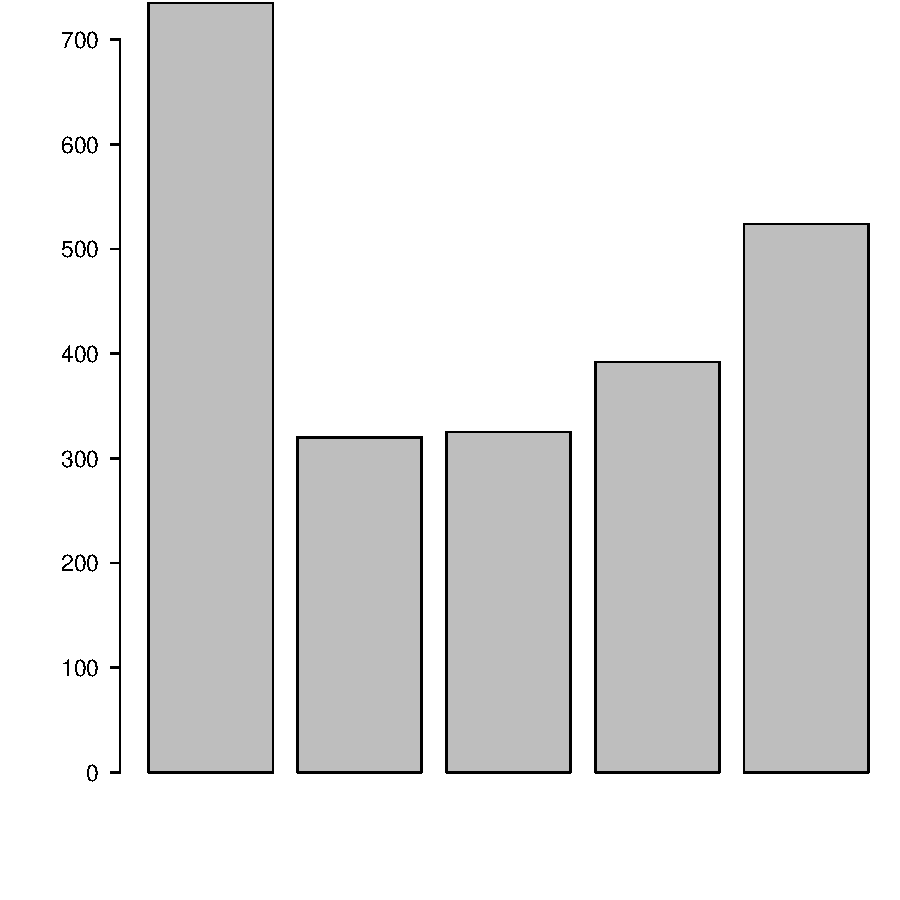
\includegraphics[width=.6\linewidth]{figure/Meng51940633A1-Rnwauto-report-1} 

}


\begin{kframe}\begin{alltt}
\hlcom{#Answer: No, it is not recorded in a decreasing order.}

\hlcom{#e.}
\hlstd{Rivers} \hlkwb{<-} \hlkwd{sort}\hlstd{(rivers,} \hlkwc{decreasing} \hlstd{=} \hlnum{TRUE}\hlstd{)}
\hlkwd{barplot}\hlstd{(Rivers[}\hlnum{1}\hlopt{:}\hlnum{10}\hlstd{])}
\end{alltt}
\end{kframe}

{\centering 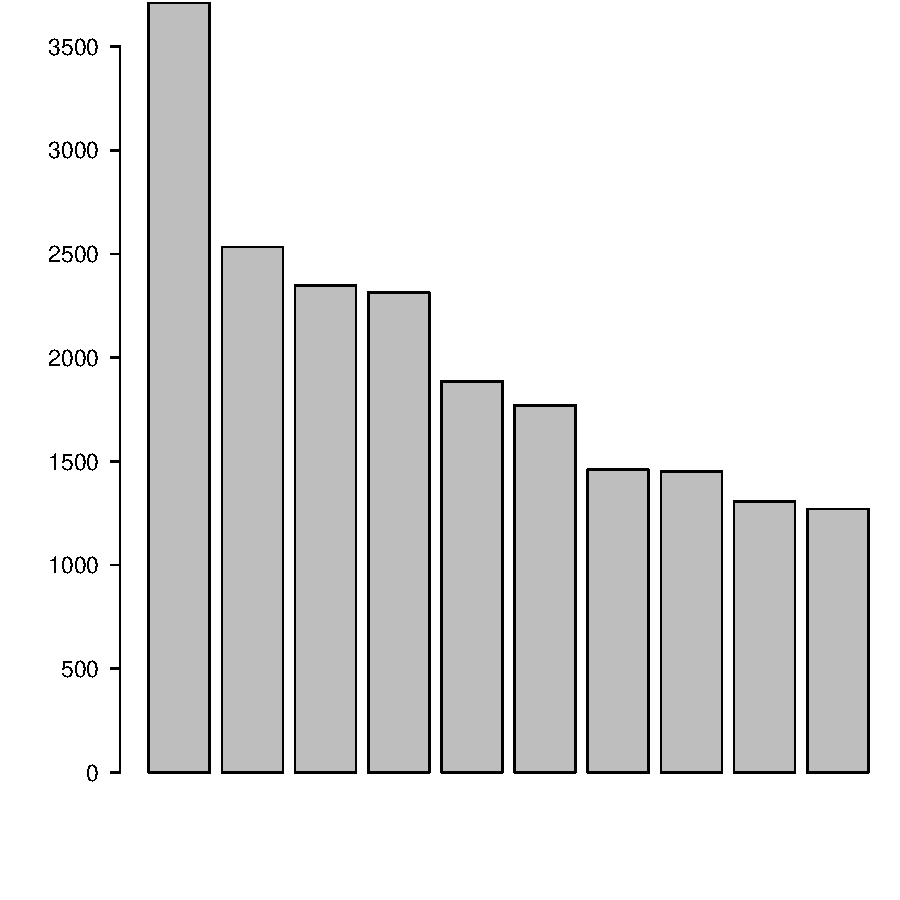
\includegraphics[width=.6\linewidth]{figure/Meng51940633A1-Rnwauto-report-2} 

}


\begin{kframe}\begin{alltt}
\hlcom{#Answer: There are 4 rivers that are longer than 2000 miles.}

\hlcom{#f.}
\hlkwd{barplot}\hlstd{(rivers[}\hlnum{1}\hlopt{:}\hlnum{10}\hlstd{])}
\end{alltt}
\end{kframe}

{\centering 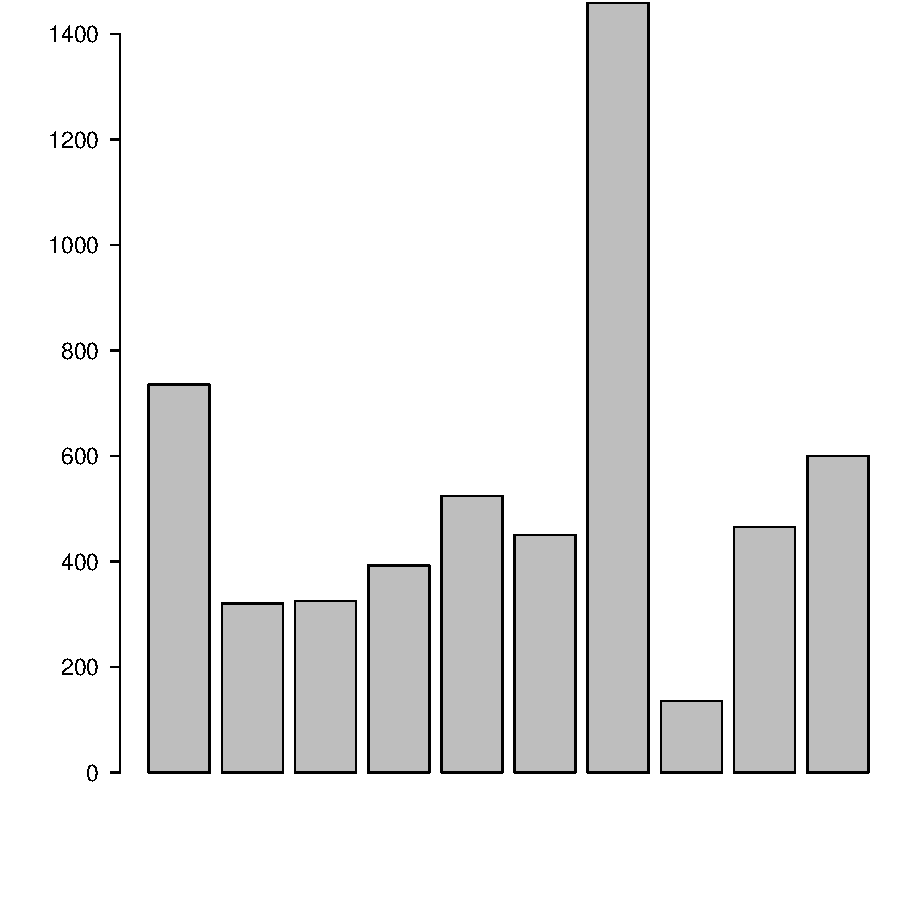
\includegraphics[width=.6\linewidth]{figure/Meng51940633A1-Rnwauto-report-3} 

}


\begin{kframe}\begin{alltt}
\hlstd{rivers[}\hlnum{1}\hlopt{:}\hlnum{10}\hlstd{]}
\end{alltt}
\begin{verbatim}
##  [1]  735  320  325  392  524  450 1459  135  465  600
\end{verbatim}
\begin{alltt}
\hlcom{#Answer: There are 0 river that are longer than 2000 miles.}

\hlcom{#g.}
\hlcom{#Answer: There are 0 river that are longer than 1500 miles.}

\hlcom{#h.}
\hlcom{#Answer: There are 3 rivers that are longer than 500 miles.}

\hlcom{##Question 3}

\hlcom{#3a. Generate this code pattern: }
\hlcom{## [1] 1 4 9 16 25 36 49 64 81 100}
\hlcom{#Answer is:}
\hlstd{(}\hlnum{1}\hlopt{:}\hlnum{10}\hlstd{)}\hlopt{^}\hlnum{2}
\end{alltt}
\begin{verbatim}
##  [1]   1   4   9  16  25  36  49  64  81 100
\end{verbatim}
\begin{alltt}
\hlcom{#3b. Generate this code pattern:}
\hlcom{## [1] 2 4 6 8 10 12 14 16 18 20 22 24 26 28 30 32}
\hlcom{## [17] 34 36 38 40 42 44 46 48 50 52 54 56 58 60 62 64}
\hlcom{## [33] 66 68 70 72 74 76 78 80 82 84 86 88 90 92 94 96}
\hlcom{## [49] 98 100}
\hlcom{#Answer is:}
\hlkwd{seq}\hlstd{(}\hlnum{2}\hlstd{,} \hlnum{100}\hlstd{,} \hlnum{2}\hlstd{)}
\end{alltt}
\begin{verbatim}
##  [1]   2   4   6   8  10  12  14  16  18  20  22  24  26  28  30  32  34  36  38  40  42
## [22]  44  46  48  50  52  54  56  58  60  62  64  66  68  70  72  74  76  78  80  82  84
## [43]  86  88  90  92  94  96  98 100
\end{verbatim}
\begin{alltt}
\hlcom{#3c.}
\hlcom{#Answer:}
\hlstd{n} \hlkwb{<-} \hlnum{1}\hlopt{:}\hlnum{5}
\hlstd{an} \hlkwb{<-} \hlnum{1} \hlopt{-} \hlstd{(}\hlnum{1}\hlopt{/}\hlstd{n)}
\hlstd{an} \hlcom{#[1] 0.0000000 0.5000000 0.6666667 0.7500000 0.8000000}
\end{alltt}
\begin{verbatim}
## [1] 0.000000000000000 0.500000000000000 0.666666666666667 0.750000000000000
## [5] 0.800000000000000
\end{verbatim}
\begin{alltt}
\hlcom{#3d. }
\hlcom{#Answer:}
\hlstd{n} \hlkwb{<-} \hlnum{5}
\hlstd{an} \hlkwb{<-} \hlnum{1} \hlopt{-} \hlstd{(}\hlnum{1}\hlopt{/}\hlstd{n)}
\hlstd{an} \hlcom{#[1] 0.8}
\end{alltt}
\begin{verbatim}
## [1] 0.8
\end{verbatim}
\begin{alltt}
\hlcom{# it seems that R gave me a much less sig fig number for this one.}


\hlcom{#3e.}
\hlcom{#Answer:}
\hlcom{#i: }
\hlkwd{sum}\hlstd{(}\hlnum{1}\hlopt{:}\hlnum{200}\hlstd{)} \hlcom{#[1] 20100}
\end{alltt}
\begin{verbatim}
## [1] 20100
\end{verbatim}
\begin{alltt}
\hlcom{#ii:}
\hlstd{nVec} \hlkwb{=} \hlnum{1}\hlopt{:}\hlnum{20}
\hlstd{GLseq} \hlkwb{<-} \hlstd{(}\hlopt{-}\hlnum{1}\hlstd{)}\hlopt{^}\hlstd{(nVec}\hlopt{+}\hlnum{1}\hlstd{)}\hlopt{/}\hlstd{(}\hlnum{2}\hlopt{*}\hlstd{nVec}\hlopt{-}\hlnum{1}\hlstd{)}
\hlkwd{sum}\hlstd{(GLseq)} \hlcom{#[1] 0.772906}
\end{alltt}
\begin{verbatim}
## [1] 0.77290595166696
\end{verbatim}
\begin{alltt}
\hlstd{pi}\hlopt{/}\hlnum{4} \hlcom{#[1] 0.7853982}
\end{alltt}
\begin{verbatim}
## [1] 0.785398163397448
\end{verbatim}
\begin{alltt}
\hlstd{nVec2} \hlkwb{=} \hlnum{1}\hlopt{:}\hlnum{100}
\hlstd{GLseq} \hlkwb{<-} \hlstd{(}\hlopt{-}\hlnum{1}\hlstd{)}\hlopt{^}\hlstd{(nVec2}\hlopt{+}\hlnum{1}\hlstd{)}\hlopt{/}\hlstd{(}\hlnum{2}\hlopt{*}\hlstd{nVec2}\hlopt{-}\hlnum{1}\hlstd{)}
\hlkwd{sum}\hlstd{(GLseq)} \hlcom{#[1] 0.7828982}
\end{alltt}
\begin{verbatim}
## [1] 0.782898225889638
\end{verbatim}
\begin{alltt}
\hlstd{pi}\hlopt{/}\hlnum{4} \hlcom{#[1] 0.7853982}
\end{alltt}
\begin{verbatim}
## [1] 0.785398163397448
\end{verbatim}
\begin{alltt}
\hlstd{nVec2} \hlkwb{=} \hlnum{1}\hlopt{:}\hlnum{1000}
\hlstd{GLseq} \hlkwb{<-} \hlstd{(}\hlopt{-}\hlnum{1}\hlstd{)}\hlopt{^}\hlstd{(nVec2}\hlopt{+}\hlnum{1}\hlstd{)}\hlopt{/}\hlstd{(}\hlnum{2}\hlopt{*}\hlstd{nVec2}\hlopt{-}\hlnum{1}\hlstd{)}
\hlkwd{sum}\hlstd{(GLseq)} \hlcom{#[1] 0.7851482}
\end{alltt}
\begin{verbatim}
## [1] 0.785148163459948
\end{verbatim}
\begin{alltt}
\hlstd{pi}\hlopt{/}\hlnum{4} \hlcom{#[1] 0.7853982}
\end{alltt}
\begin{verbatim}
## [1] 0.785398163397448
\end{verbatim}
\begin{alltt}
\hlstd{nVec2} \hlkwb{=} \hlnum{1}\hlopt{:}\hlnum{10000}
\hlstd{GLseq} \hlkwb{<-} \hlstd{(}\hlopt{-}\hlnum{1}\hlstd{)}\hlopt{^}\hlstd{(nVec2}\hlopt{+}\hlnum{1}\hlstd{)}\hlopt{/}\hlstd{(}\hlnum{2}\hlopt{*}\hlstd{nVec2}\hlopt{-}\hlnum{1}\hlstd{)}
\hlkwd{sum}\hlstd{(GLseq)} \hlcom{#[1] 0.7853732}
\end{alltt}
\begin{verbatim}
## [1] 0.785373163397511
\end{verbatim}
\begin{alltt}
\hlstd{pi}\hlopt{/}\hlnum{4} \hlcom{#[1] 0.7853982}
\end{alltt}
\begin{verbatim}
## [1] 0.785398163397448
\end{verbatim}
\begin{alltt}
\hlstd{nVec2} \hlkwb{=} \hlnum{1}\hlopt{:}\hlnum{100000}
\hlstd{GLseq} \hlkwb{<-} \hlstd{(}\hlopt{-}\hlnum{1}\hlstd{)}\hlopt{^}\hlstd{(nVec2}\hlopt{+}\hlnum{1}\hlstd{)}\hlopt{/}\hlstd{(}\hlnum{2}\hlopt{*}\hlstd{nVec2}\hlopt{-}\hlnum{1}\hlstd{)}
\hlkwd{sum}\hlstd{(GLseq)} \hlcom{#[1] 0.7853957}
\end{alltt}
\begin{verbatim}
## [1] 0.785395663397448
\end{verbatim}
\begin{alltt}
\hlstd{pi}\hlopt{/}\hlnum{4} \hlcom{#[1] 0.7853982}
\end{alltt}
\begin{verbatim}
## [1] 0.785398163397448
\end{verbatim}
\begin{alltt}
\hlstd{nVec2} \hlkwb{=} \hlnum{1}\hlopt{:}\hlnum{1000000}
\hlstd{GLseq} \hlkwb{<-} \hlstd{(}\hlopt{-}\hlnum{1}\hlstd{)}\hlopt{^}\hlstd{(nVec2}\hlopt{+}\hlnum{1}\hlstd{)}\hlopt{/}\hlstd{(}\hlnum{2}\hlopt{*}\hlstd{nVec2}\hlopt{-}\hlnum{1}\hlstd{)}
\hlkwd{sum}\hlstd{(GLseq)} \hlcom{#[1] 0.7853979}
\end{alltt}
\begin{verbatim}
## [1] 0.785397913397448
\end{verbatim}
\begin{alltt}
\hlstd{pi}\hlopt{/}\hlnum{4} \hlcom{#[1] 0.7853982}
\end{alltt}
\begin{verbatim}
## [1] 0.785398163397448
\end{verbatim}
\begin{alltt}
\hlcom{#Answer: as n is from 1:higher & higher number, we can expect the Gregory formula to simplify}
\hlcom{#closer to pi/4.}

\hlcom{#3f.}
\hlcom{#Answer}
\hlcom{#i:}
\hlstd{vec} \hlkwb{=} \hlkwd{rep}\hlstd{(}\hlkwd{c}\hlstd{(}\hlnum{5}\hlopt{:}\hlnum{1}\hlstd{,}\hlnum{1}\hlopt{:}\hlnum{5}\hlstd{),}\hlnum{10}\hlstd{)}
\hlkwd{rep}\hlstd{(}\hlkwd{seq}\hlstd{(}\hlnum{1}\hlstd{,}\hlnum{100}\hlstd{), vec)}
\end{alltt}
\begin{verbatim}
##   [1]   1   1   1   1   1   2   2   2   2   3   3   3   4   4   5   6   7   7   8   8   8
##  [22]   9   9   9   9  10  10  10  10  10  11  11  11  11  11  12  12  12  12  13  13  13
##  [43]  14  14  15  16  17  17  18  18  18  19  19  19  19  20  20  20  20  20  21  21  21
##  [64]  21  21  22  22  22  22  23  23  23  24  24  25  26  27  27  28  28  28  29  29  29
##  [85]  29  30  30  30  30  30  31  31  31  31  31  32  32  32  32  33  33  33  34  34  35
## [106]  36  37  37  38  38  38  39  39  39  39  40  40  40  40  40  41  41  41  41  41  42
## [127]  42  42  42  43  43  43  44  44  45  46  47  47  48  48  48  49  49  49  49  50  50
## [148]  50  50  50  51  51  51  51  51  52  52  52  52  53  53  53  54  54  55  56  57  57
## [169]  58  58  58  59  59  59  59  60  60  60  60  60  61  61  61  61  61  62  62  62  62
## [190]  63  63  63  64  64  65  66  67  67  68  68  68  69  69  69  69  70  70  70  70  70
## [211]  71  71  71  71  71  72  72  72  72  73  73  73  74  74  75  76  77  77  78  78  78
## [232]  79  79  79  79  80  80  80  80  80  81  81  81  81  81  82  82  82  82  83  83  83
## [253]  84  84  85  86  87  87  88  88  88  89  89  89  89  90  90  90  90  90  91  91  91
## [274]  91  91  92  92  92  92  93  93  93  94  94  95  96  97  97  98  98  98  99  99  99
## [295]  99 100 100 100 100 100
\end{verbatim}
\begin{alltt}
\hlcom{#ii: }
\hlnum{2}\hlopt{^}\hlstd{(}\hlkwd{seq}\hlstd{(}\hlnum{0}\hlstd{,}\hlnum{8}\hlstd{))}
\end{alltt}
\begin{verbatim}
## [1]   1   2   4   8  16  32  64 128 256
\end{verbatim}
\begin{alltt}
\hlcom{#iii:}
\hlkwd{rep}\hlstd{(}\hlkwd{rep}\hlstd{(}\hlkwd{seq}\hlstd{(}\hlnum{3}\hlstd{,}\hlnum{7}\hlstd{),}\hlkwd{c}\hlstd{(}\hlnum{3}\hlstd{,}\hlnum{2}\hlstd{,}\hlnum{4}\hlstd{,}\hlnum{2}\hlstd{,}\hlnum{1}\hlstd{)),}\hlnum{5}\hlstd{)}
\end{alltt}
\begin{verbatim}
##  [1] 3 3 3 4 4 5 5 5 5 6 6 7 3 3 3 4 4 5 5 5 5 6 6 7 3 3 3 4 4 5 5 5 5 6 6 7 3 3 3 4 4 5 5
## [44] 5 5 6 6 7 3 3 3 4 4 5 5 5 5 6 6 7
\end{verbatim}
\begin{alltt}
\hlcom{#iv:}
\hlkwd{seq}\hlstd{(}\hlopt{-}\hlnum{6}\hlstd{,}\hlnum{21}\hlstd{,}\hlkwc{by}\hlstd{=}\hlnum{3}\hlstd{)}
\end{alltt}
\begin{verbatim}
##  [1] -6 -3  0  3  6  9 12 15 18 21
\end{verbatim}
\end{kframe}
\end{knitrout}

The R session information (including the OS info, R version and all
packages used):

\begin{knitrout}
\definecolor{shadecolor}{rgb}{0.969, 0.969, 0.969}\color{fgcolor}\begin{kframe}
\begin{alltt}
\hlkwd{sessionInfo}\hlstd{()}
\end{alltt}
\begin{verbatim}
## R version 4.2.2 (2022-10-31)
## Platform: x86_64-apple-darwin17.0 (64-bit)
## Running under: macOS Ventura 13.1
## 
## Matrix products: default
## LAPACK: /Library/Frameworks/R.framework/Versions/4.2/Resources/lib/libRlapack.dylib
## 
## locale:
## [1] en_US.UTF-8/en_US.UTF-8/en_US.UTF-8/C/en_US.UTF-8/en_US.UTF-8
## 
## attached base packages:
## [1] stats     graphics  grDevices utils     datasets  methods   base     
## 
## loaded via a namespace (and not attached):
##  [1] compiler_4.2.2  magrittr_2.0.3  tools_4.2.2     glue_1.6.2      vctrs_0.5.1    
##  [6] stringi_1.7.8   highr_0.10      knitr_1.41      stringr_1.5.0   xfun_0.36      
## [11] lifecycle_1.0.3 rlang_1.0.6     evaluate_0.19
\end{verbatim}
\begin{alltt}
\hlkwd{Sys.time}\hlstd{()}
\end{alltt}
\begin{verbatim}
## [1] "2023-02-01 09:29:26 PST"
\end{verbatim}
\end{kframe}
\end{knitrout}


\end{document}
